\documentclass{article}


% This file is a solution template for:
% 1 inch margins
\usepackage{fullpage}

\usepackage{booktabs}
\usepackage{longtable}

\usepackage{hyperref}
\usepackage{graphicx}
\usepackage{multicol}
\usepackage{subcaption}

% Add ability to resume enumeration environments with /begin{enumerate}[resume]
\usepackage{enumitem}

\usepackage{pgf}
\usepackage{tikz}
\usepackage{bodegraph}
\usepackage{circuitikz}
\usetikzlibrary{calc}
\usetikzlibrary{trees}
\usetikzlibrary{arrows}
\usetikzlibrary{shapes}
\usetikzlibrary{fadings}
\usetikzlibrary{positioning}
\usetikzlibrary{intersections}


\usepackage[english]{babel}
\usepackage[latin1]{inputenc}
\usepackage[T1]{fontenc}
% Or whatever. Note that the encoding and the font should match. If T1 does not look nice, try deleting the line with the fontenc.


\usepackage{listings}

\usepackage{amsmath}


\usepackage{xspace}
\newcommand{\Ohm}{$\Omega$\xspace}



\title{Feedback and PID Control Theory}


\tikzstyle{block} = [draw, fill=blue!20, rectangle, 
    minimum height=3em, minimum width=6em]
\tikzstyle{sum} = [draw, fill=blue!20, circle, node distance=1cm]
\tikzstyle{input} = [coordinate]
\tikzstyle{output} = [coordinate]
\tikzstyle{pinstyle} = [pin edge={to-,thin,black}]

\begin{document}
\maketitle

\section{Introduction}
Feedback is a mechanism for regulating a physical system so that it maintains a certain state. Feedback works by measuring the current state of a physical system, determining how far the current state is from the desired state, and then automatically applying a control signal to bring the system closer to the desired state. This process is repeated iteratively to bring the system to the desired state and keep it there.

Feedback can be used very effectively to stabilize the state of a system, while also improving its performance: Engineers use feedback to control otherwise unstable designs; op amps use feedback to stabilize and linearize their gain; and physicists use feedback to stabilize and improve the performance of their instruments.

\subsection{Feedback in engineering}
Feedback is ubiquitous in engineering. Its application has led to device features and machines which would not otherwise function. Here are few examples.

\paragraph{Climate control} A sensor measures the temperature and humidity in a room and then heats or cools and humidifies or dehumidifies accordingly.

\paragraph{Automobile cruise control} The car measures its speed and then applies the accelerator or not depending on whether the speed must be increased or decreased to maintain the target speed.

\paragraph{Highly maneuverable fighter jets} The F-16 Falcon fighter jet is an inherently unstable aircraft (i.e. the airframe will not glide on its own). The F-16 does fly because 5 onboard computers constantly measure the aircraft's flight characteristics and then apply corrections to the control surfaces (i.e. rudder, flaps, ailerons, etc\ldots) to keep it from tumbling out of control. The advantage of this technique is that the aircraft has the very rapid response and maneuverability of a naturally unstable airframe, while also being able to fly.


\subsection{Feedback in electronics}
Op-amps use feedback to achieve very high linearity and predictability for their closed-loop gain by sacrificing some of their extremely high open-loop gain.

Another common application of feedback in electronics is in precision, fast- response power supplies. Constant current and constant voltage power supplies which have a high degree of stability use feedback to regulate their current or their voltage, by measuring the current and voltage across a precision shunt resistor and then using feedback to automatically correct for any deviations from the desired output. Feedback also allows the power supply to adjust its voltage or current very quickly and controllably in response to a change in load.

\subsection{Feedback in physics}
Feedback has become a familiar tool for experimental physicists to improve the stability of their instruments. In particular, physicists use feedback for precise control of temperature, for stabilizing and cooling particle beams in accelerators, for improving the performance of atomic force microscopes, for locking the optical frequency of lasers to atomic transitions, and referencing quartz oscillators to ground state atomic hyperfine microwave transitions in atomic clocks, to name just a few example.

\paragraph{Temperature control} Many delicate physics devices, such as crystals, lasers, RF oscillators, and amplifiers, require their temperature to be very stable in order to guarantee their performance. For example, the wavelength of diode lasers generally has a temperature dependence on the order of 0.2\,nm/$^\circ$C, but requires a stability of $10^{-6}$\,nm for experiments.

\paragraph{Stochastic cooling} In a particle accelerator, the transverse momentum spread of particles must be reduced to a minimum. The reduced momentum spread increases the particle density, or beam luminosity, and consequently the probability of collisions with a similar counter-propagating particle beam in the detector area. Stochastic cooling works by measuring the transverse positions and momenta of the particles as they pass through a section of the accelerator, and then applying appropriate momentum kicks to some of the particles at other points in the accelerator ring to reduce the overall transverse momentum spread. The process is repeated until the momentum spread is sufficiently reduced. The 1984 Nobel Prize in Physics was awarded in part to Simon van der Meer for his invention of stochastic cooling which contributed to the discovery of the $W$ and $Z$ bosons (weak force mediators) at CERN.

\paragraph{Atomic force microscope} An atomic force microscope uses a very sharp tip (just a few nanometers in size at the very tip) which is scanned back and forth just a few nanometers above the surface to be imaged. Instead of scanning the tip at a constant height above the surface, which could lead to the tip actually running into a bump on the surface, the microscope uses feedback to adjust the tip height such that the force (from the surface atoms) on the tip is constant.

\paragraph{Laser locking} Many experiments in atomic and optical physics require lasers which have a very stable optical frequency. The optical frequency of the laser is locked by measuring the optical frequency difference between the laser and an atomic transition and using feedback to set this difference to a constant value. Lasers can be routinely stabilized with feedback to better than 1\,MHz out of $3 \times 10^{14}$\,Hz (about 1 part per billion), though stabilities close to 1\,Hz have been reported after heroic efforts.

\paragraph{Atomic clocks} In an atomic clock, the frequency of an RF oscillator (a quartz crystal for example) is compared to that of a ground state atomic hyperfine microwave transition (6.8 or 9.2\,GHz). The frequency difference is measured and the frequency of the RF oscillator is corrected by feedback. The process is constantly repeated to eliminate any drift in the frequency of the RF oscillator. Atomic fountain clocks can achieve accuracies in the range of 1 part in $10^{15}$, and plans are underway to construct optical atomic clocks with accuracies and stabilities of about 1 part in $10^{18}$.

\section{Feedback}
In this section we introduce the main elements of a generic feedback model.

\begin{figure}
 \begin{center}
  \begin{tikzpicture}[auto, node distance=2cm,>=latex']
    % http://www.texample.net/tikz/examples/control-system-principles/
    % We start by placing the blocks
    %\node [input, name=input] {};
    %\node [sum, right of=input] (sum) {};
    \node [block] (controller) {Controller};
    \node [block, right of=controller, pin={[pinstyle]above:Disturbances $v$},
            node distance=3cm] (system) {System $S$};
    % We draw an edge between the controller and system block to 
    % calculate the coordinate u. We need it to place the measurement block. 
    \draw [->] (controller) -- node[name=u] {$u$} (system);
    \node [output, right of=system] (output) {};
    \node [block, below of=u] (measurements) {Measurements};
    % Once the nodes are placed, connecting them is easy. 
    %\draw [draw,->] (input) -- node {$r$} (sum);
    %\draw [->] (sum) -- node {$e$} (controller);
    \draw [->] (system) -- node [name=y] {$y$}(output);
    \draw [->] (y) |- (measurements);
    %\draw [->] (measurements) -| node[pos=0.99] {$-$} 
    %    node [near end] {$y_m$} (sum);
  \end{tikzpicture}
 \end{center}
\caption{Conceptual schematic of a system.}
\label{fig:block_diagram_system_no_feedback}
\end{figure}

\subsection{System}
Consider a simple system characterized by a single variable $S$. Under normal conditions the system is in a steady state $S = S_0$ which may vary and drift somewhat over time due to the variation of environmental variables $v$ which we cannot measure or are unaware of. We possess a mechanism for measuring the output $y$ of the system\footnotemark{} as well as a control input $u$ which we can use to modify the state $S$ of the system. In summary, the system has the following functional form $y = S(u; v; t)$. We will make the final assumption that $S$ is monotonic with $u$ in the vicinity of $S_0$ (i.e. that the plot of $S$ vs.~$u$ does not have any maxima or minima, and that $dS/du$ is either always positive or always negative).

\footnotetext{Our measurements are generally denoted as $y_m$ since they may not be a direct measurement of the output $y$ of the system.  However, for the purpose of this discussion, we will assume that we can directly measure the state of the system, and thus $y_m = y$.}

Figure~\ref{fig:block_diagram_system_no_feedback} shows a conceptual schematic of the relationship between the system, the variables $u$ and $v$, and the output $y$ of the system state $S$.

\subsection{Objective}
Our objective is to set or lock the state of the system to a desired value $S = S_d$ and keep it there without letting it drift or vary over time, regardless of variations in the environmental variables $v$.

\begin{figure}
 \begin{center}
  \begin{tikzpicture}[auto, node distance=2cm,>=latex']
    % http://www.texample.net/tikz/examples/control-system-principles/
    % We start by placing the blocks
    \node [input, name=input] {};
    \node [sum, right of=input] (sum) {};
    \node [block, right of=sum] (controller) {Controller};
    \node [block, right of=controller, pin={[pinstyle]above:Disturbances $v$},
            node distance=3cm] (system) {System $S$};
    % We draw an edge between the controller and system block to 
    % calculate the coordinate u. We need it to place the measurement block. 
    \draw [->] (controller) -- node[name=u] {$u$} (system);
    \node [output, right of=system] (output) {};
    \node [block, below of=u] (measurements) {Measurements};
    % Once the nodes are placed, connecting them is easy. 
    \draw [draw,->] (input) -- node {$y_d$} (sum);
    \draw [->] (sum) -- node {$e$} (controller);
    \draw [->] (system) -- node [name=y] {$y$}(output);
    \draw [->] (y) |- (measurements);
    \draw [->] (measurements) -| node[pos=0.99] {$-$} 
        node [near end] {$y_m$} (sum);
  \end{tikzpicture}
 \end{center}
\caption{Conceptual schematic of a system with the feedback loop.}
\label{fig:block_diagram_system_with_feedback}
\end{figure}

\subsection{Feedback model}
We will set or lock the state of the system to $S = S_d$ and corresponding $y = y_d$ with the following procedure (see also Figure~\ref{fig:block_diagram_system_with_feedback}):
\begin{enumerate}
\item \label{enum:measure} Measure the state $S$ of the system.
\item Determine how far the system is from its desired set point by defining an error variable, $e = y - y_d$.
\item Calculate a trial control value $u = u(e)$.
\item Feed the calculated control value, $u(e)$, back into the control input of the system $S$.
\item \label{enum:change} The state of the system changes in response to the change in the control value.
\item Return to step \ref{enum:measure}.
\end{enumerate}

If we repeat this feedback cycle indefinitely with an appropriately calculated control value $u(e)$, then the system will converge to the state $S = S_d$ and remain there even under the influence of small changes to other variables (i.e. $v$) which influence the value of the state $S$.

This feedback model can be adapted to include several state variables and several feedback variables.

In section~\ref{sec:PID_feedback_control}, we discuss a frequently used expression for calculating the feedback control variable $u(e)$.


\section{PID Feedback Control}
\label{sec:PID_feedback_control}
The most popular type of feedback stabilization control, $u(e)$, is Proportional-Integral-Derivative (PID) gain feedback. PID is very effective and easy to implement. The expression for $u(e)$ depends only on the error signal $e = y - y_d$ and is given by
\begin{equation}
u(e;t) = g_P e(t) + g_I \int_0^t e(t)dt + g_D \frac{d}{dt} e(t),
\end{equation}
where $g_P$, $g_I$, and $g_D$ are respectively the proportional, integral, and derivative gains. We also note that $g_P$, $g_I$, and $g_D$ do not have the same units. We will assume for simplicity that $g_P$ is dimensionless in which case $u(e)$ has the same units as $e$.

\subsection{Time evolution of the system with PID feedback control}
We are now in a position to calculate the time evolution of the system under the influence of feedback. Without feedback, the system would remain in the state $S_0$:	
\begin{equation}
S_{no~feedback}(t) = S_0.
\end{equation}
$S_0$ may vary in time, but we will ignore this effect until part \ref{sec:time_evolution:solution}.

In the presence of feedback, the state of the system at time $t + \Delta t$ (step~\ref{enum:change}) depends on the state of the system without feedback, $S_0$, which has been modified by the control input variable $u(e)$. We now make the following simplifying assumption that the control input variable, $u(e)$, ``controls'' or modifies the state of the system $S$ through the process of addition. In this case, the system state variable $S$ evolves according to the following equation:
\begin{equation}
S(t+\Delta t) = S_0 + u(e;t). \label{eqn:step}
\end{equation}
We can convert this equation to an integro-differential equation, if we assume that the system has a characteristic response time $\tau$ (small).  In this case, equation~\ref{eqn:step} becomes
\begin{equation}
S(t) + \tau \frac{d}{dt} S(t) = S_0 + g_P e(t) + g_I \int_0^t e(t)dt + g_D \frac{d}{dt} e(t). \label{eqn:full_diff_eq}
\end{equation}


\subsection{Special case: pure proportional gain feedback}
As a limiting case we consider pure proportional gain feedback ($g_I = 0$ and $g_D = 0$). We study this special case, because it is the basis for op amp feedback and is also the simplest form of feedback. For $g_I = 0$ and $g_D = 0$, equation~\ref{eqn:full_diff_eq} becomes
\begin{equation}
S(t) + \tau \frac{d}{dt} S(t) = S_0 + g_P e(t). \label{eqn:proportional_only_diff_eq}
\end{equation}
We can solve this 1st order differential equation, for the initial condition $S(t=0) = S_0$, with the same technique we used in the determination of the time evolution of the voltage on a charging capacitor. After a little bit of integration and algebra, which is left as an exercise to the reader, we find the following solution:
\begin{equation}
S(t) = \left(S_0 - \frac{S_0 - g_P S_d}{1 - g_P}\right) e^{-(1-g_P)t/\tau} + \frac{S_0 - g_P S_d}{1 - g_P}. \label{eqn:proportional_only_solution}
\end{equation}
Equation~\ref{eqn:proportional_only_solution} shows that the system will converge to the state $S = (S_0 - g_P S_d) / (1 - g_P)$ when feedback control is applied, so long as the exponential exponent is negative (i.e. $g_P < 1$), otherwise $S$ will diverge. We note that $g_P < 0$ corresponds to negative feedback.

Figure~\ref{fig:P_from_05_to_1} shows the response of a system for a dimensionless gain of $g_P = -10$ and state values $S_0 = 0.5$ and $S_d = 1$, with time measured in units of $\tau$ (the system characteristic response time).

\begin{figure}
\begin{center}
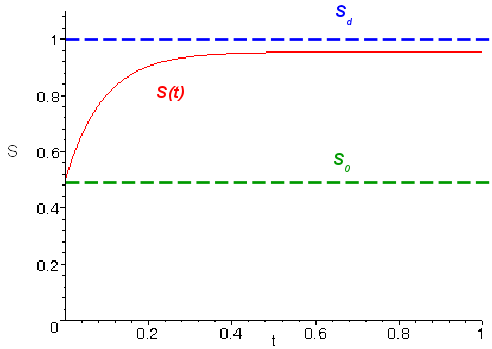
\includegraphics[width=0.4\textwidth]{pics/P_from_05_to_1}
\end{center}
\caption{System response with pure proportional gain feedback control and parameters $g_P = -10$, $S_0 = 0.5$, and $S d = 1$. Time is measure in units of $\tau$ (the system characteristic response time).}
\label{fig:P_from_05_to_1}
\end{figure}

As Figure~\ref{fig:P_from_05_to_1} makes clear, the system does not converge to the desired state $S = S_d$, though it does reach its final steady state value relatively quickly. If we restrict ourselves to negative feedback, then according to equation~\ref{eqn:proportional_only_solution}, the system will converge to the steady state value $S_{ss}$ of 
\begin{equation}
S_{ss} = \frac{S_0 - g_P S_d}{1 - g_P}.
\end{equation}
Equation~\ref{eqn:proportional_only_solution} indicates that the system can be made to converge to a steady state value $S_{ss}$ which is arbitrarily close to $S = S_d$ just by increasing the gain. In fact, for infinite negative proportional gain (i.e $g_P \to -\infty$) the system does converge to $S_{ss} = S_d$: this is the limit in which op amp feedback operates.

A note of caution: On its own, equation~\ref{eqn:proportional_only_solution} is a little misleading since it would seem to imply that large positive feedback, $g_P \to +\infty$, would also produce $S_{ss} = S_d$. Of course, this is not true since according to equation~\ref{eqn:proportional_only_diff_eq}, the system will never achieve a steady state, but instead will diverge forever.

\subsection{Solution for PI feedback control}
\label{sec:time_evolution:solution}

A large majority of PID feedback controllers are actually just PI controllers (i.e. proportional and integral gain, but no derivative gain), and so for simplicity we solve equation~\ref{eqn:full_diff_eq} without the derivative gain term ($g_D = 0$). The inclusion of the derivative gain term is conceptually simple and follows the same treatment as PI feedback and is left as an exercise to reader. Derivative gain is used to improve the time response of the feedback, so that the system converges more quickly to its steady state value.

With the derivative gain term omitted, equation~\ref{eqn:full_diff_eq} becomes
\begin{equation}
S(t) + \tau \frac{d}{dt} S(t) = S_0 + g_P e(t) + g_I \int_0^t e(t)dt.
\end{equation}
We can convert this integro-differential equation to a 2nd order linear differential equation with constant coefficients by taking the time derivative of this equation to obtain
\begin{equation}
\frac{d}{dt} S(t) + \tau \frac{d^2}{dt^2} S(t) = g_P \frac{d}{dt} S + g_I (S - S_d),
\end{equation}
where we employed the substitution $e(t) = S - S_d$. After combining similar terms, this equation becomes
\begin{equation}
\tau \frac{d^2}{dt^2} S(t) + (1 - g_P) \frac{d}{dt} S(t) - g_I S(t) = - g_I S_d. \label{eqn:proportional_integral_diff_eq}
\end{equation}
This is an inhomogeneous 2nd order differential equation with constant coefficients. The full solution to this differential equation is given by
\begin{eqnarray}
S(t) & = & A_+ e^{\lambda_+ t} + A_- e^{\lambda_- t} + S_d, \label{eqn:proportional_integral_solution} \\
\lambda_\pm & = & \frac{(g_P - 1) \pm \sqrt{(g_P - 1)^2 + 4 g_I \tau}}{2 \tau}.
\end{eqnarray}
The first two terms of equation~\ref{eqn:proportional_integral_solution} represent the homogeneous solution to equation~\ref{eqn:proportional_integral_diff_eq}, while the 3rd term is the inhomogeneous solution to the equation (it does not depend on the initial conditions).  The coefficients $A_+$ and $A_-$ are constants to be determined from the initial conditions.

Equation~\ref{eqn:proportional_integral_solution} shows that the system will converge to the state $S = S_d$ when feedback control is applied, so long as $\lambda_+$ and $\lambda_-$ are negative (i.e. negative feedback), otherwise $S$ will diverge (exactly the opposite of what we want to accomplish with feedback).

If we choose $S(t=0) = S_0$ and $dS(t=0)/dt = 0$ as our initial conditions, we can calculate the constants $A^+$ and $A^-$. After a little bit of algebra, we find that
\begin{eqnarray}
A_+ & = & - \frac{\lambda_-}{\lambda_- - \lambda_+} (S_d - S_0), \\
A_- & = & \frac{\lambda_+}{\lambda_- - \lambda_+} (S_d - S_0).
\end{eqnarray}
In Figure~\ref{fig:PI_from_05_to_1}, the behavior of the system under PI feedback control is plotted for several different parameters configurations.

\begin{figure}
\begin{center}
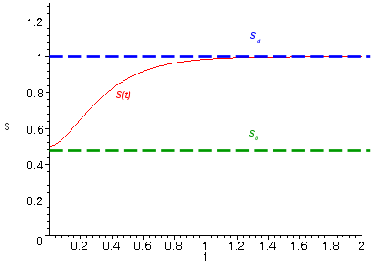
\includegraphics[width=0.4\textwidth]{pics/PI_from_05_to_1_settings1}
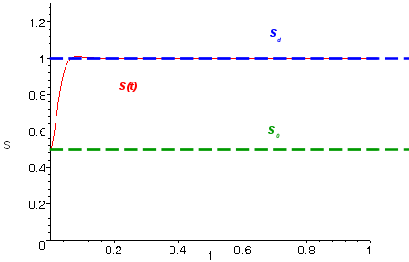
\includegraphics[width=0.4\textwidth]{pics/PI_from_05_to_1_settings2}
\end{center}
\caption{Time-evolution of a generic system with PI control feedback for $S_0 = 0.5$ and $S_d = 1$. For the left hand plot the gain parameters are $g_P = -10$, $g_I = -30$, while for the right hand plot the parameters are $g_P = -100$, $g_I = -4000$. The small overshoot in the left hand plot is due to a small imaginary part in the exponential exponent of equation~\ref{eqn:proportional_integral_solution}.}
\label{fig:PI_from_05_to_1}
\end{figure}

The primary purpose of integral gain is to provide essentially infinite gain at DC (0\,Hz), which guarantees that $S_{ss} = S_d$, as can be seen in Figure~\ref{fig:PI_from_05_to_1}. Figure~\ref{fig:PI_from_05_to_1} also shows that the larger the gain, the faster the correction time of the feedback control loop.

\subsection{Fourier space analysis of noise suppression}
One of the primary objectives of feedback is to make the system insensitive to noise on the system state $S$, so that the system state stays locked to $S = S_d$ regardless of external influences.

In the absence of corrective feedback, external noise will cause the system state to deviate from $S = S_0$. External noise at a frequency $\omega$ will cause the system state to oscillate around its natural steady state such that $S = S_0 + S_N \cos\omega t$, where $S_N$ is the amplitude of the oscillations. Following the standard Fourier space recipe, we replace $\cos\omega t$ with $\exp i\omega t$, and then take the real part at the end of our calculations. In essence, we must re-solve the differential equation with the following modification:
\begin{equation}
S_0 \to S_0 + S_N e^{i\omega t}
\end{equation}
After substitution, equation~\ref{eqn:proportional_integral_diff_eq} becomes
\begin{equation}
\tau \frac{d^2}{dt^2} S(t) + (1 - g_P) \frac{d}{dt} S(t) - g_I S = i\omega S_N e^{i\omega t} - g_I S_d. \label{eqn:proportional_integral_diff_eq_with_noise}
\end{equation}
Equation~\ref{eqn:proportional_integral_diff_eq_with_noise} has the same homogeneous solution as equation~\ref{eqn:proportional_integral_diff_eq}, but the inhomogeneous solution, $S_{ih}(t)$, differs and is given by the following expression
\begin{equation}
S_{ih}(t) = \frac{i\omega}{(1 - g_P) i\omega - \tau \omega^2 - g_I} S_N  e^{i\omega t} + S_d.
\end{equation}
We see that the noise term is present in the inhomogeneous solution, but with an additional factor modifying the amplitude of the noise. In the case of negative feedback the modulus of this suppression factor, which we will call $A_N$, is always less than unity and is given by the following expression
\begin{equation}
A_N = \frac{\omega}{\sqrt{(1 - g_P)^2 \omega^2 + (\tau \omega^2 + g_I)^2}}.
\end{equation}

The plot in figure~\ref{fig:PI_noise_suppression} shows the dependence of the suppression factor, $A_N$, on frequency for different feedback schemes. The plot shows that a combination of proportional and integral control gives the best suppression of noise, except in the vicinity of the ``resonant'' frequency $\omega = \sqrt{-g_I/\tau}$. The high frequency drop-off of the suppression factor is not due to feedback but simply the natural response time $\tau$ of the system which also suppresses noise.

\begin{figure}
\begin{center}
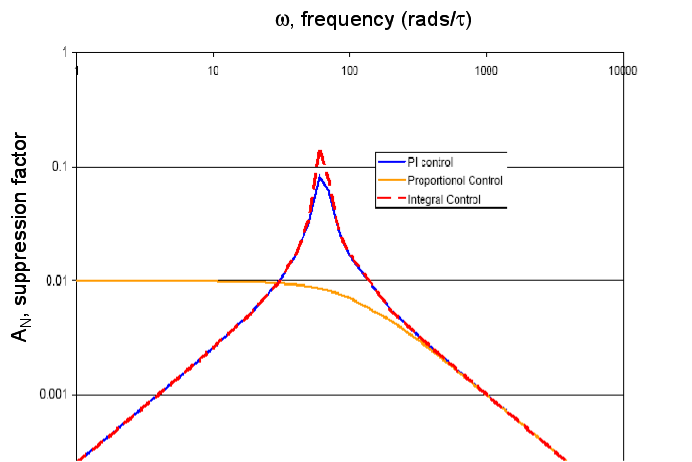
\includegraphics[width=0.4\textwidth]{pics/PI_noise_suppression}
\end{center}
\caption{Comparison of the suppression factor, $A_N$, for different feedback schemes. The feedback control loop parameters are $g_P = -100$ and $g_I = -4000$.}
\label{fig:PI_noise_suppression}
\end{figure}

\section{Reality}
In practice, feedback is not quite as straightforward as presented in the previous section. 

\subsection{Gain vs.~Frequency}
In the theoretical treatment of part~\ref{sec:PID_feedback_control}, we assumed that the proportional gain was independent of frequency. In practice, gain will generally fall off at higher frequencies due to natural low-pass $RC$ filtering in an amplifier and the larger circuit.

As an example, Figure~\ref{fig:OP27_open_loop_gain} shows a plot of the open-loop gain of an op amp as function of frequency, which has a clear drop-off in gain at higher frequencies.

\begin{figure}
\begin{center}
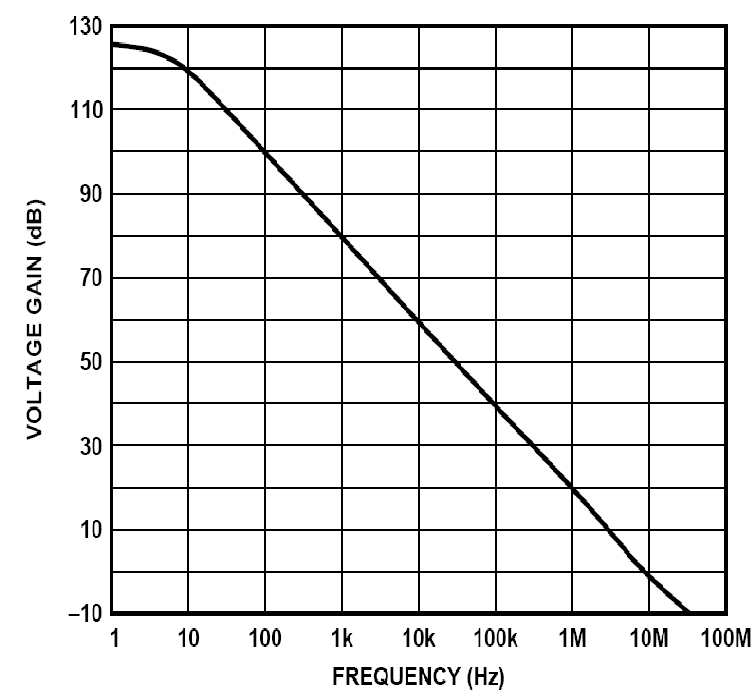
\includegraphics[width=0.4\textwidth]{pics/OP27_open_loop_gain}
\end{center}
\caption{Open-loop gain of the OP27 op amp (Analog Devices OP27 datasheet revision F, p. 10 (2006)).}
\label{fig:OP27_open_loop_gain}
\end{figure}

\subsection{Phase shifts and positive feedback}
The natural or stray $RC$ filtering of an amplifier not only rolls off the gain at high frequencies, but also introduces a $-\pi/2$ phase shift. If the feedback loop has a second stray unintentional $RC$ filter present (for example, the natural time response of the system), then a second $-\pi/2$ phase shift is introduced. If the feedback gain is larger than 1 at the frequency at which the total accumulated phase is $-\pi$, then the feedback loop goes into positive feedback which causes the state of the system to diverge or sometimes oscillate out of control.

\subsection{Stray $RC$ positive feedback compensation}
One way to avoid having the system go into positive feedback is to purposely introduce an additional $RC$ low-pass filter into the feedback loop. If this $RC$ filter has a $f_{3dB}$ frequency which is sufficiently smaller than the frequency at which the positive feedback occurs then the attenuation of the filter can bring the gain below 1 when the $-\pi$ phase shift occurs. This way the feedback loop will no longer go into positive feedback above a certain frequency (of course there will not be any noise suppression or feedback action above this frequency either).


\pagebreak

\section{Design Exercises}

\begin{figure}
\begin{center}
\begin{circuitikz}
\draw (0,0) node[op amp](opamp){};
\draw (-1.2,-1) node[ground]{} |- (opamp.+);
\draw (-2.5,-1) node[ground]{} to[photodiode,i^<=$i_{PD,reverse}$] ++(0,+1.5) |- (opamp.-);
\draw (opamp.out) to[short,-o] ++(0.5,0) node[right]{$v_{out}$};
\draw (opamp.out) node[circ]{} to[short] ++(0,1.5) to[R,l=$R$] ++(-2,0) -| (opamp.-) node[circ]{};
\end{circuitikz}
\end{center}
\caption{Photodiode with an op amp current-to-voltage inverting amplifier.}
\label{fig:photodiode_opamp}
\end{figure}

\begin{enumerate}
\item \label{ex:pid_feedback} Consider an LED facing a photodiode in a manner similar to what you did last week when you constructed the photodiode circuits. Design a circuit which will maintain a constant optical power incident on the photodiode, even in the presence of external fluctuations in the room lighting. You should use the op amp circuit of figure~\ref{fig:photodiode_opamp} and use PI feedback control to stabilize the intensity of the LED. Your circuit should be able to provide at least 10\,mA at $\sim 2$\,V to the LED.

\begin{figure}
\begin{center}
\begin{circuitikz}
\draw (0,0) node[op amp](opamp){};
\draw (opamp.-) to[R,l=$R_1$] ++(-2,0) node[ground]{};
\draw (opamp.+) to[short,-o] ++(-0.5,0) node[left]{$v_{in}$};
\draw (opamp.out) to[short,-o] ++(0.5,0) node[right]{$v_{out}$};
\draw (opamp.out) to[short] ++(0,1.5) to[R,l=$R_2$] ++(-2,0) -| (opamp.-);
\end{circuitikz}
\end{center}
\caption{Non-inverting amplifier.}
\label{fig:non_inverting_amplifier}
\end{figure}

\item The non-inverting op amp amplifier with finite open-loop gain.

In this exercise you will NOT use the op amp golden rules to solve the problem, unless explicitly indicated.  Consider the non-inverting op amp amplifier in the circuit in Figure~\ref{fig:non_inverting_amplifier}.  In the following parts, $v^+$ and $v^-$ refer respectively to the voltages at the non-inverting and inverting terminals of the op amp. The open-loop gain of the op amp is $A$.
\begin{enumerate}
\item Write down the fundamental op amp relation between $v^+$, $v^-$, $v_{out}$, and $A$ when no feedback is present (i.e. when $R_1$ and $R_2$ are not present).
\item Assuming that the $v^-$ input draws no current, derive an expression for $v^-$ in terms of $v_{out}$, $R_1$, and $R_2$.
\item Obtain an expression for $v_{out}$ in terms of $v_{in}$, $A$, $R_1$, and $R_2$, and determine the gain $G$ of the amplifier. Calculate $v_{out}$ in the limit of $A \to +\infty$ Calculate $v_{out}$ in the limit $A \to -\infty$ and comment on its physical meaning.
\item Suppose that the open-loop gain, $A$, is not very constant with frequency and changes by $\Delta A$ between frequencies $f_1$ and $f_2$. Derive an expression for the resulting relative variation in the amplifier gain $\Delta G / G$ in terms of the relative variation in the open-loop gain $\Delta A / A$. Calculate $\Delta G / G$ and $\Delta A / A$ for $A = 10^6$, $\Delta A = 10^5$,  $R_2 = 100$\,k\Ohm, and $R_1 = 10$\,k\Ohm.
\item Most op amps feature a significant drop-off in their open-loop gain at frequencies above $\sim 10$\,Hz. The drop-off follows a well established curve given by $A \cdot f = constant$, where the constant is called the gain-bandwidth product ($f$ is frequency in Hz). The gain-bandwidth product of the OP27 is 8\,MHz. On the same log-log graph, plot the open-loop gain $A$ vs. frequency and the closed loop gain $G$ vs. frequency (for $R_2 = 100$\,k\Ohm and $R_1 = 10$\,k\Ohm) for an OP27-based non-inverting amplifier.
\end{enumerate}
\end{enumerate}

\section{Lab: PI Feedback Control}

This week's lab focuses on the use of PI feedback control to stabilize the incident light on a photodiode. We also introduce the Peltier thermoelectric cooler which is frequently used for precision temperature control in electronic circuits.

\begin{enumerate}
\item PI feedback control of an LED (2.5 hours \ldots infinite if you are not prepared)

Construct the light blinker with a LED and a function generator like we did before. Construct the transimpedance amplifier of Figure~\ref{fig:photodiode_opamp} to convert a photodiode current to voltage, use a 100\,k\Ohm feedback resistor. Use your circuit design from design exercise~\ref{ex:pid_feedback} to regulate the optical power incident on the photodiode despite of the disturbance introduced by the blinker. The circuit should be such that the incident optical power can be set with some control resistor.

Recommendations:
\begin{enumerate}
\item Choose the desired light level: measure the output of the photodiode plus op amp detector circuit (with LED on at about desired level), and set $V_{ctrl}$ (i.e. $S_d$) to between 0\,V and the highest measured values, i.e. make desired values within the reach of the system.
\item Integrator starting values: $R = 1$\,k\Ohm, $C = 100$\,nF, $R_f = 10$\,M\Ohm.
\item Proportional gain range: $0 < g_P < 10$ (adjustable with a potentiometer).
\item Procedure: Build at test each of the schematics parts separately, link them and test them consequently as you are linking them together. Make sure that outputs behave the way they should.
\item Necessary but not sufficient check: Link all together but put the light controlling LED away from the photodiode, make your blinker frequency a few Hz, the light controlling LED must blink out of phase with the one driven by the function generator.
\item Gain adjustments: Put your light controlling LED so it shines on the photodiode. Adjust gains so it makes the error signal a flat line at 0\,V. Start off with only integral gain (zero out or remove proportional gain), and then once you get negative feedback, you can slowly add in the proportional gain to optimize the response.
\end{enumerate}

Questions:
\begin{enumerate}
\item Determine experimentally the integral and proportional gain that you need in order for the feedback to function properly.
\item Use a second LED attached to a square-wave generator to see how fast your circuit can respond and modify the intensity of its LED to keep incident optical power on the photodiode constant. Adjust the integral and proportional gain to optimize the response time of your feedback circuit. What is the fastest response time that you can obtain with your circuit? How does the feedback control respond to a step function change in incident optical power from an external source (an oscilloscope plot will suffice)?
\item If you increase the proportional gain sufficiently, the feedback loop will go into positive feedback and start to oscillate uncontrollably. What is the frequency of this oscillation?
\end{enumerate}

\item (Bonus) Adapt your PI feedback control circuit to regulate the temperature of a Peltier thermoelectric cooler using the thermometer circuit you built in a previous lab.

\end{enumerate}

\end{document}
